\documentclass{article}

\usepackage[final]{project}

\usepackage[utf8]{inputenc}
\usepackage[T1]{fontenc}
\usepackage{hyperref}
\usepackage{url}
\usepackage{booktabs}
\usepackage{amsfonts}
\usepackage{nicefrac}
\usepackage{microtype}
\usepackage{caption}
\usepackage{subcaption}
\usepackage{amsmath}
\usepackage{amssymb}
\usepackage{graphicx}

\title{Can Phase-Conditioned Imitation Recover Biomechanically Realistic Gait? \\ A Walker2d Case Study}

\author{%
  Brock Pereca \\
  Kahlert School of Computing \\
  University of Utah \\
  \texttt{brock.perreca@gmail.com} \\
  \And
  Brian Keller \\
  Kahlert School of Computing \\
  University of Utah \\
}

\begin{document}

\maketitle

\begin{abstract}
Producing natural, human-like walking in physics-based simulation is difficult because hand-crafted reward functions either under-specify the desired gait---yielding reward-hacked, biomechanically implausible locomotion---or over-specify it, yielding brittle motion that requires hand-engineering the very gait one is trying to learn. We investigate, on a MuJoCo Walker2d agent conditioned on inverse-kinematics reference data from the Ulrich treadmill walking dataset (Subject 1, 1.25\,m/s), how far an engineered-reward imitation pipeline can carry us toward biomechanically realistic gait. We train a phase-conditioned PPO policy with a DeepMimic-style multi-term reward, reference-state initialization, and behavioral cloning warm-start, and evaluate the resulting policy against a held-out biomechanical-realism scorecard built from the subject's measured force-plate vertical ground reaction force (vGRF) and IK joint kinematics. Training is stable and produces visually plausible bipedal locomotion. The held-out scorecard, however, finds that the policy systematically violates the kinetic structure of human walking: peak vGRF reaches 3--4 body weights versus a measured reference of 1.10 BW, double-support fraction collapses to roughly 1\,\% versus the measured 23\,\%, and joint range of motion under-shoots the reference by 30--50\,\% at the hip and ankle. The policy walks the way the reward was written, not the way humans walk. We additionally implement Adversarial Motion Priors (AMP) and AIRL as a comparison and confirm the discriminator collapse mechanism that prevents AMP from training at small environment counts. Together these findings indicate that engineered-reward imitation on a 2D torque-actuated planar biped is not sufficient for biomechanically realistic gait, and motivate two complementary paths forward: GPU-parallelized adversarial imitation, and a return to the muscle-actuated dynamics of the original proposal.
\end{abstract}

\section{Introduction}

A central challenge in physics-based character animation, embodied AI, and biomechanical modeling is the gait imitation problem: given a reference motion captured from a human subject, train a reinforcement learning policy to reproduce that motion in a rigid-body simulation subject to gravity, contact, and actuator constraints. The downstream motivation is concrete. Assistive-device design, prosthetic and exoskeleton control, and musculoskeletal modeling all rely on simulated locomotion that is mechanically consistent with recorded human movement; if the simulator's gait is biomechanically implausible, every conclusion drawn from it inherits the implausibility.

The original ambition of this project was a lab-to-field comparison study: train 3D, muscle-actuated agents on lab-grade marker, force-plate, and EMG references versus markerless smartphone OpenCap~\cite{uhlrich2023opencap} references, and measure the loss in emergent biomechanical fidelity (vGRF, EMG activations, joint contact forces) when the cheaper sensing modality replaces the expensive one. That study was scoped down to a tractable backup question: \emph{can the imitation pipeline that question depends on actually produce biomechanically realistic gait in the first place?} If the answer is no on a simpler, faster benchmark, the lab-versus-field comparison cannot be answered cleanly on the harder one.

We investigate this question on the MuJoCo Walker2d-v4 planar biped, a well-studied torque-actuated benchmark with 8 degrees of freedom (six actuated joints: bilateral hip, knee, and ankle). Our reference motion is derived from inverse-kinematics reconstruction of treadmill walking from the Ulrich dataset (Subject 1, 1.25\,m/s), processed into a single clean gait cycle of 140 frames at 50\,Hz, then resampled to 350 frames at 125\,Hz via cubic spline to match the simulator control rate. We use a custom Walker2d MJCF whose hip joint range admits the full reference flexion peak.

This project sits at the intersection of model-free RL (PPO~\cite{schulman2017ppo}), imitation learning (behavioral cloning warm-start), adversarial imitation (AMP~\cite{escontrela2022amp}, AIRL~\cite{fu2018airl}), and biomechanical evaluation, making it directly relevant to the reinforcement learning methods covered in this course. The reward-hacking failure modes we document are canonical examples of Goodhart's Law in RL: when a measure becomes a target it ceases to be a good measure.

The primary contributions of this project are:
\begin{itemize}\setlength\itemsep{1pt}
    \item A working phase-conditioned PPO + DeepMimic-style imitation policy trained on real human IK data, with reference-state initialization and a PD-rollout behavioral cloning warm-start. The policy trains stably and produces bipedal locomotion that survives multi-thousand-step episodes at the target speed.
    \item A held-out \emph{biomechanical-realism scorecard} that compares each candidate policy against the subject's measured force-plate vGRF and IK joint kinematics, scoring per-metric \% deviation and an aggregate progress score in $[0,4]$. The scorecard is decoupled from the training reward and exposes the gap between visual plausibility and biomechanical realism.
    \item Empirical evidence that the engineered DeepMimic-reward pipeline produces visually plausible policies that systematically fail biomechanical realism on the kinetic axes the reward leaves unspecified: peak vGRF, double-support fraction, and joint ROM amplitude.
    \item A taxonomy of structured reward-hacking failure modes encountered during reward engineering, framed as Goodhart cases.
    \item A faithful implementation of AMP and AIRL on top of the same observation and dynamics, and a mechanistic characterization of AMP's discriminator collapse at the 8-environment CPU scale.
\end{itemize}

\section{Related Work}

\textbf{DeepMimic}~\cite{peng2018deepmimic} introduced the motion imitation paradigm for physics-based characters: a phase-indexed reference clip drives a dense reward composed of weighted exponential penalties on pose, velocity, end-effector, and root-tracking errors. Our reward design follows this framework, including the reference-state initialization (RSI) scheme in which episodes are reset to a uniformly sampled reference frame. DeepMimic operated on articulated 3D humanoids; we apply the same principles to the planar Walker2d benchmark with real human IK data, and crucially evaluate the resulting policy against \emph{measured} biomechanical targets rather than against training-time return.

\textbf{Adversarial Motion Priors}~\cite{escontrela2022amp} replaced hand-crafted style reward terms with a learned LSGAN discriminator trained on expert motion transitions, combined with a small task reward via $r = w_g r_{\text{task}} + w_s r_{\text{style}}$. Their key enabling condition is massive environment parallelism (4096 environments on a GPU cluster), which prevents discriminator collapse. We implement AMP faithfully but are constrained to 8 CPU environments, producing the collapse behavior characterized in Section~\ref{sec:results-amp}.

\textbf{AIRL}~\cite{fu2018airl} learns a disentangled reward function with a shaping potential $f(s,s') + \gamma h(s') - h(s)$. We implement AIRL as a sibling to AMP for comparison; the shaping term partially mitigates the discriminator-saturation failure mode but does not avoid it at small scale.

\textbf{Massively Parallel Deep RL}~\cite{rudin2022walk} demonstrated that GPU-parallelized environments (4096 environments on a single GPU) reduce wall-clock training time for legged locomotion from hours to minutes. Their work directly motivates our planned migration to MuJoCo MJX (JAX GPU backend) as the natural next step for AMP, where discriminator coverage requires policy diversity achievable only with thousands of simultaneous rollouts.

\textbf{PPO}~\cite{schulman2017ppo} is our base RL algorithm throughout, via Stable Baselines~3. PPO's on-policy nature is well-matched to the dense, phase-dependent reward landscape of gait imitation, where off-policy value estimates from stale experience cause catastrophic forgetting of phase alignment.

\textbf{Dynamic Time Warping}~\cite{kovar2002motiongraphs} provides a sequence-alignment metric robust to temporal phase offset between motion clips. We use DTW distance between the agent's full-episode joint trajectory and the reference cycle as one component of the held-out evaluation scorecard, to capture shape fidelity independently of minor phase drift.

\textbf{Musculoskeletal simulation.} The MyoSuite framework~\cite{caggiano2022myosuite} provides a 3D, 80-muscle, 20-DoF musculoskeletal lower-body model that was the platform of our original proposal. We return to this thread in Section~\ref{sec:conclusion}: the negative result on torque-actuated 2D imitation strengthens the case that biomechanical realism is more naturally enforced by physiological dynamics than by reward weights.

\section{Problem Statement}

We formalize gait imitation as a Markov Decision Process $\mathcal{M} = (\mathcal{S}, \mathcal{A}, \mathcal{T}, r, \gamma)$ augmented with a reference motion and a held-out biomechanical evaluation.

\paragraph{State.} Let $q \in \mathbb{R}^{8}$ be the generalized positions (excluding global $x$-translation) and $\dot q \in \mathbb{R}^{9}$ the generalized velocities of the Walker2d. The base simulator observation is $s_{\text{base}} = [q, \dot q] \in \mathbb{R}^{17}$.

\paragraph{Reference motion.} A reference gait cycle is a sequence of joint configurations $\mathcal{R} = \{q^{\text{ref}}_t\}_{t=0}^{T-1}$, $q^{\text{ref}}_t \in \mathbb{R}^{6}$, representing the hip, knee, and ankle angles (bilateral) of a human walking at 1.25\,m/s, sampled at the simulator control frequency. The cycle is periodic: $q^{\text{ref}}_T = q^{\text{ref}}_0$.

\paragraph{Phase.} A scalar phase index $\phi \in \{0, \ldots, T-1\}$ advances by one per environment step, wrapping modulo $T$. The phase-conditioned observation augments the base state:
\[
s = [\, s_{\text{base}} \mid q^{\text{ref}}_\phi \mid \sin(2\pi\phi/T) \mid \cos(2\pi\phi/T) \,] \in \mathbb{R}^{25}.
\]

\paragraph{Training objective.} The agent finds a policy $\pi^*$ maximizing the expected discounted return
\[
\pi^* = \arg\max_\pi \; \mathbb{E}_{\tau \sim \pi}\!\left[\sum_{t=0}^{\infty} \gamma^t\, r(s_t, a_t, \phi_t) \right],
\]
where $r$ encodes fidelity to the reference motion and $\phi_t = t \bmod T$.

\paragraph{Held-out biomechanical realism.} Distinct from the training reward, we define a held-out evaluation against measured human gait. Let $\mathcal{B}^{\text{ref}} = \{T_{\text{stride}}^*, \mathrm{DSF}^*, \mathrm{vGRF}^*_{\text{peak}}, \mathrm{ROM}^*_j\}$ be biomechanical targets computed directly from Subject 1's force-plate signals and IK joint angles. For each policy rollout we compute the matched quantities $\mathcal{B}^{\pi}$ from the simulator and report per-metric \% deviation $|b^\pi - b^*| / b^*$ together with an aggregate progress score in $[0, 4]$. The training reward never sees $\mathcal{B}$. A policy that achieves high return while $\mathcal{B}^\pi$ deviates substantially from $\mathcal{B}^{\text{ref}}$ has reward-hacked the imitation objective.

\section{Method}
\label{sec:method}

\subsection{Phase-conditioned observation and reference-state initialization}

The Walker2d-v4 default observation is phase-blind: the policy sees joint angles and velocities but has no information about where it is in the gait cycle. We augment the observation with $q^{\text{ref}}_\phi$ and $(\sin\phi, \cos\phi)$ as defined above. At episode reset, RSI samples a uniformly random phase $\phi_0 \sim \mathrm{Uniform}(0, T)$ and initializes joint angles and velocities to the reference values at that phase, with forward velocity initialized to the target $\dot q_0 = 1.25$\,m/s. The forward-velocity initialization is critical: a body initialized mid-stride with zero forward velocity is in a physically inconsistent state that causes immediate failure.

\subsection{DeepMimic-style multi-term imitation reward}

Our reward is a weighted sum of six tracking terms scaled by the timestep $\Delta t$:
\[
r = r_{\text{pose}} + r_{\text{vel}} + r_{\text{ee}} + r_{\text{root}} + r_{\text{contact}} - r_{\text{swing}} + r_{\text{ctrl}}.
\]
Per-joint exponential penalties use sharpness $k_j \in \{10, 20, 40\}$ and weights $w_j \in \{0.4, 1.0, 2.5\}$ for hip, knee, and ankle respectively (ankle highest, because heel-strike timing is controlled primarily by the ankle joint). Reference joint velocities are estimated via central differences with periodic boundary conditions. Forward kinematics are precomputed at initialization to obtain reference foot positions; the swing-phase end-effector reward uses sharpness $k_z = 200$ (vs.\ $40$ at stance) to trigger earlier in toe-off and prevent toe-drag. Contact forces are extracted from MuJoCo's \texttt{cfrc\_ext}; the contact-alternation term $\tanh(F_{\text{stance}}/50) - \tanh(F_{\text{swing}}/50)$ rewards loading the reference-specified stance foot while a direct $-w_{\text{swing}} \tanh(F_{\text{swing}}/50)$ penalty closes the toe-drag exploit not caught by the alternation term. Including torso pitch in the root term prevents the ``controlled forward fall'' degenerate solution, which minimizes height error while maximizing forward speed.

\subsection{Behavioral cloning warm-start with PD rollouts}

Rather than using inverse dynamics to compute reference torques (which ignores ground reaction forces and is systematically wrong during stance), we roll out a PD tracking controller $\tau = K_p(q^{\text{ref}} - q) + K_d(\dot q^{\text{ref}} - \dot q)$ inside the full MuJoCo simulation. Because the rollout runs inside the simulator, contact forces are computed at every integration sub-step, producing torques that are physically consistent with ground contact. We collect 200{,}000 $(s, a)$ pairs and pretrain the policy network via supervised learning before RL fine-tuning.

\subsection{Adversarial Motion Priors and AIRL}

AMP replaces hand-crafted style terms with a discriminator $D_\psi: \mathbb{R}^{24} \to \mathbb{R}$ trained to distinguish reference motion transitions from policy transitions. Discriminator input is the concatenated $(s, s')$ pair in 12-dimensional joint space $[q_j, \dot q_j] \in \mathbb{R}^{12}$, giving 24 dimensions. The LSGAN discriminator loss with zero-centered gradient penalty on expert samples is
\[
\mathcal{L}_D = \mathbb{E}_{\text{expert}}\!\left[(D-1)^2\right] + \mathbb{E}_{\text{policy}}\!\left[(D+1)^2\right] + \tfrac{\lambda}{2}\, \mathbb{E}_{\text{expert}}\!\left[\lVert \nabla_s D \rVert^2 \right],
\]
with $\lambda = 10$ and additive expert noise $\sigma = 0.05$\,rad to soften the expert manifold. The bounded style reward is $r_s = \max(0,\, 1 - 0.25(D-1)^2) \in [0, 1]$, combined with a forward-velocity task reward as $r = w_g r_{\text{task}} + w_s r_s$ with $w_g = 0.35$, $w_s = 0.65$. AIRL uses the same discriminator architecture but with the disentangled reward formulation $f(s,s') + \gamma h(s') - h(s)$ to recover a transferable shaping potential.

\subsection{Held-out biomechanical evaluation}
\label{sec:method-eval}

We extract biomechanical targets directly from Subject 1's lab data: peak vertical ground reaction force per body weight from the force plate, stride period and double-support fraction from rising-edge contact detection on the force-plate signal, and joint range of motion from the IK time-series. The reference values for the baseline 1.25\,m/s trial are: stride period 1.12\,s, double-support fraction 0.227, peak vGRF/BW 1.10, and per-joint ROM (hip 45.4$^\circ$, knee 65.7$^\circ$, ankle 40.0$^\circ$).

For each candidate policy, we run six deterministic rollouts of 2500 steps each, compute the matched quantities, and report (a) per-metric \% deviation from the reference, (b) full L+R kinematics overlay against the reference cycle, (c) both-leg vGRF stance-phase curves, (d) hip--knee phase-plane comparison, and (e) an aggregate progress score in $[0, 4]$ that aggregates the per-metric deviations against a $\pm 20$\,\% credible band. Critically, none of these quantities appear in the training reward.

\section{Experimental Design}

\subsection{Hypotheses}

\textbf{H1.} A phase-conditioned PPO policy trained with the multi-term DeepMimic reward, RSI, and BC warm-start produces stable, visually plausible bipedal locomotion at the target speed of 1.25\,m/s.

\textbf{H2.} Visual plausibility does \emph{not} imply biomechanical realism. The held-out scorecard reveals systematic deviations from measured human gait on kinetic axes the training reward leaves unspecified: peak vGRF, double-support fraction, and joint ROM amplitude.

\textbf{H3.} AMP at 8 CPU environments suffers discriminator collapse: the discriminator achieves near-perfect separation early, the style reward saturates near zero, and the resulting policy is qualitatively worse than the engineered baseline.

\subsection{Domain and data}

\textbf{Simulator.} MuJoCo 3.3.0 via Gymnasium Walker2d-v4. We use a custom MJCF (\texttt{walker2d\_hipopen.xml}, \texttt{thigh\_joint range="-30 60"}) whose hip joint range admits the reference's $+30^\circ$ flexion peak; the stock MJCF's \texttt{[-150, 0]} range clips the upper half of the reference cycle and produces a stiff-hip basin no reward shape can escape. Control frequency 125\,Hz, integration step 0.002\,s.

\textbf{Reference motion.} IK reconstruction of Subject 1, Ulrich treadmill walking dataset, baseline trial at 1.25\,m/s. A single clean gait cycle of 140 frames at 50\,Hz was extracted (discarding inter-trial boundaries) and resampled to 350 frames at 125\,Hz via cubic-spline interpolation.

\textbf{Policy network.} MLP with two hidden layers of 256 units, tanh activations (SB3 default). AMP discriminator: two hidden layers of 64 units, ELU activations.

\textbf{Training.} 8 parallel CPU environments (\texttt{SubprocVecEnv}), 5\,M environment steps for the PPO baseline. PPO hyperparameters: \texttt{n\_steps}=2048, batch size 64, $n_{\text{epochs}}{=}10$, $\gamma{=}0.99$, $\lambda_{\text{GAE}}{=}0.95$, learning rate $3{\times}10^{-4}$.

\subsection{Experiments}

\textbf{Experiment 1 (H1) ---} Train phase-conditioned PPO with the full multi-term reward. Evaluate via training curves (return + episode length), visual inspection of rendered episodes, and survival of deterministic 2500-step rollouts.

\textbf{Experiment 2 (H2) ---} Run the held-out biomechanical scorecard on the Experiment 1 policy. Compare measured (vGRF, DSF, ROM) against the reference. The hypothesis is confirmed if any of the metrics deviates substantially from the reference despite stable training and plausible-looking video.

\textbf{Experiment 3 (H3) ---} Train AMP at the same 8-environment scale for 20\,M steps. Evaluate by tracking the style reward over training and rendering the final policy.

\section{Results and Discussion}

\subsection{Phase-conditioned PPO trains stably (H1 confirmed)}
\label{sec:results-h1}

Figure~\ref{fig:training-curves} shows the training trajectory of the lead policy over 5\,M environment steps. Mean episodic return rises smoothly from near-zero to roughly 2{,}200, and mean episode length reaches roughly 3{,}600 steps (28.8\,s of simulated time at 125\,Hz). On six deterministic evaluation rollouts of 2500 steps each, the policy survives every episode. Visually, the policy produces bipedal locomotion at the target speed of 1.25\,m/s with bilateral foot alternation, an upright torso, and identifiable heel-strike events at each stance transition. By the standard visual criteria for ``did it learn to walk,'' the answer is yes.

\begin{figure}[t]
\centering
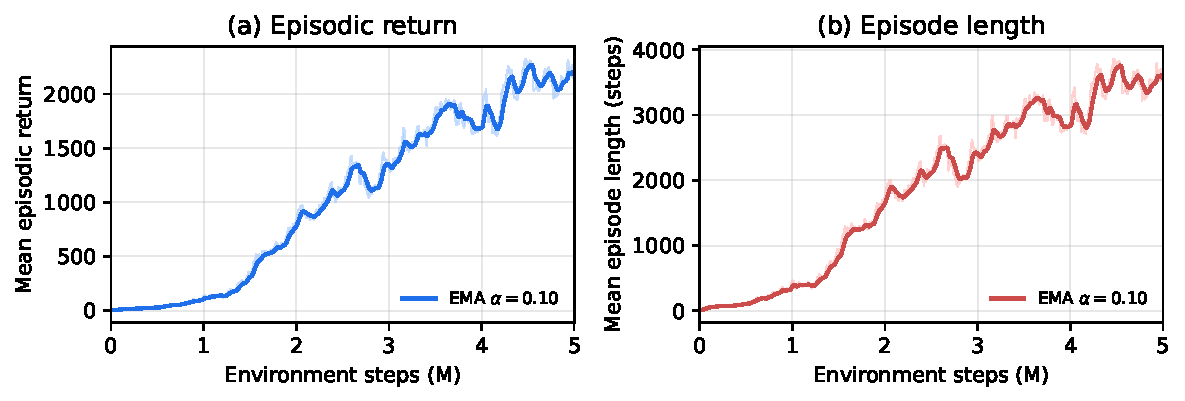
\includegraphics[width=0.92\textwidth]{fig2_training_curves.pdf}
\caption{Training curves for the lead phase-conditioned PPO policy over 5\,M environment steps. Mean episodic return (left) and episode length (right) rise smoothly and monotonically; light EMA smoothing ($\alpha = 0.10$) overlaid on raw values. The policy survives multi-thousand-step deterministic rollouts at the target speed.}
\label{fig:training-curves}
\end{figure}

\subsection{Reward-hacking failure modes encountered (Goodhart taxonomy)}
\label{sec:results-h2-exploits}

Reaching the policy in Section~\ref{sec:results-h1} required iterative reward refinement driven by visual inspection. At each stage, the optimizer found a degenerate strategy that was locally optimal for the partial reward while violating gait conventions. Each failure mode corresponds to a specific unconstrained degree of freedom (Table~\ref{tab:exploits}).

\begin{table}[t]
\caption{Reward-hacking failure modes encountered during reward design. Each is a canonical Goodhart case: the policy maximizes the partial reward by exploiting a degree of freedom that was unconstrained by the reward as written.}
\label{tab:exploits}
\centering
\small
\begin{tabular}{p{0.18\textwidth} p{0.42\textwidth} p{0.34\textwidth}}
\toprule
\textbf{Exploit} & \textbf{Mechanism} & \textbf{Closing patch} \\
\midrule
Ankle paddling & Reference ankle oscillates regardless of foot contact, so rapid ankle motion alone satisfies the joint-tracking reward with no forward progress. & Direct swing-foot contact penalty $-w_{\text{swing}}\tanh(F_{\text{swing}}/50)$. \\
\addlinespace[2pt]
One-legged hopping & Planting one foot and using the other as a balance pole satisfies stance-leg pose tracking without requiring bilateral coordination. & Explicit contact-alternation reward keyed to the reference stance foot. \\
\addlinespace[2pt]
Toe-walking & Permanent ankle plantarflexion satisfies the ankle-pose reward by walking on the toes. & End-effector tracking on foot world position. \\
\addlinespace[2pt]
Controlled forward fall & The agent leans forward to maximize $\dot x$ while staying above the height termination threshold until the lean is irrecoverable. & Pitch magnitude included in the root-tracking term and pitch-magnitude termination. \\
\addlinespace[2pt]
Stiff-hip stand & With stock MJCF's $[-150^\circ, 0^\circ]$ thigh range, the hip parks at the $+0^\circ$ wall (reference asks for $+30^\circ$) and the policy minimizes the unreachable error by holding still. & Open the MJCF thigh range to admit the reference flexion peak. \\
\bottomrule
\end{tabular}
\end{table}

These exploits are not pathological behavior from the optimizer---each is a reasonable local solution to the reward as written. They motivate both the full multi-term reward and the use of held-out biomechanical metrics in Section~\ref{sec:results-h2}, since a policy can collect high return while exhibiting any of these strategies if the reward weights are miscalibrated.

\subsection{Biomechanical realism is not recovered (H2 confirmed)}
\label{sec:results-h2}

Figure~\ref{fig:dashboard} presents the held-out biomechanical-realism scorecard for the lead policy and four comparison candidates against Subject 1's measured baseline at 1.25\,m/s. \emph{Visually plausible} and \emph{biomechanically realistic} are not the same thing. Three findings stand out, all on dimensions the multi-term reward leaves unspecified.

\textbf{Joint kinematics qualitatively track but amplitudes systematically under-shoot the reference.} The hip and ankle traces (top row of Fig.~\ref{fig:dashboard}) follow the right shape and frequency, but per-stride hip ROM lands at roughly $30^\circ$ versus the measured $45^\circ$ ($-33$\,\%), and ankle ROM at $20$--$26^\circ$ versus $40^\circ$ ($-34$ to $-51$\,\%). Knee ROM is the closest match, within $\pm 10$\,\% of the $66^\circ$ reference. The kinematic-tracking reward pulls the policy toward the reference shape but settles in a lower-amplitude basin where the residual tracking error is balanced against whatever the policy is doing on the kinetic axes the reward does not see.

\textbf{Peak vertical ground reaction force is 3--4 body weights, three to four times the reference.} The reference vGRF peaks at 1.10 BW, in line with established human walking data; every candidate policy peaks between 3.7 and 4.8 BW (Fig.~\ref{fig:dashboard}, vGRF panels). This is impact slamming, not loading: the policy lands its swing leg with enough vertical velocity to spike the contact force, then leaves the stance phase before the body can transfer weight smoothly. The multi-term reward includes a contact-alternation term but no constraint on contact-force magnitude, and the policy escapes accordingly.

\textbf{Double-support fraction collapses to roughly 1\,\%.} Walking has substantial double-support phase ($\sim 23$\,\% of the gait cycle, when both feet contact the ground simultaneously during weight transfer). Running has zero. The lead candidate sits at 0.7\,\% DSF; every other candidate is below 2.1\,\%. Combined with the high vGRF, this is unambiguously a bouncing or skipping gait, not a walking one. The reward incentivizes which foot should be loaded at each phase; it does not incentivize \emph{both} feet being loaded during transitions.

\begin{figure}[t]
\centering
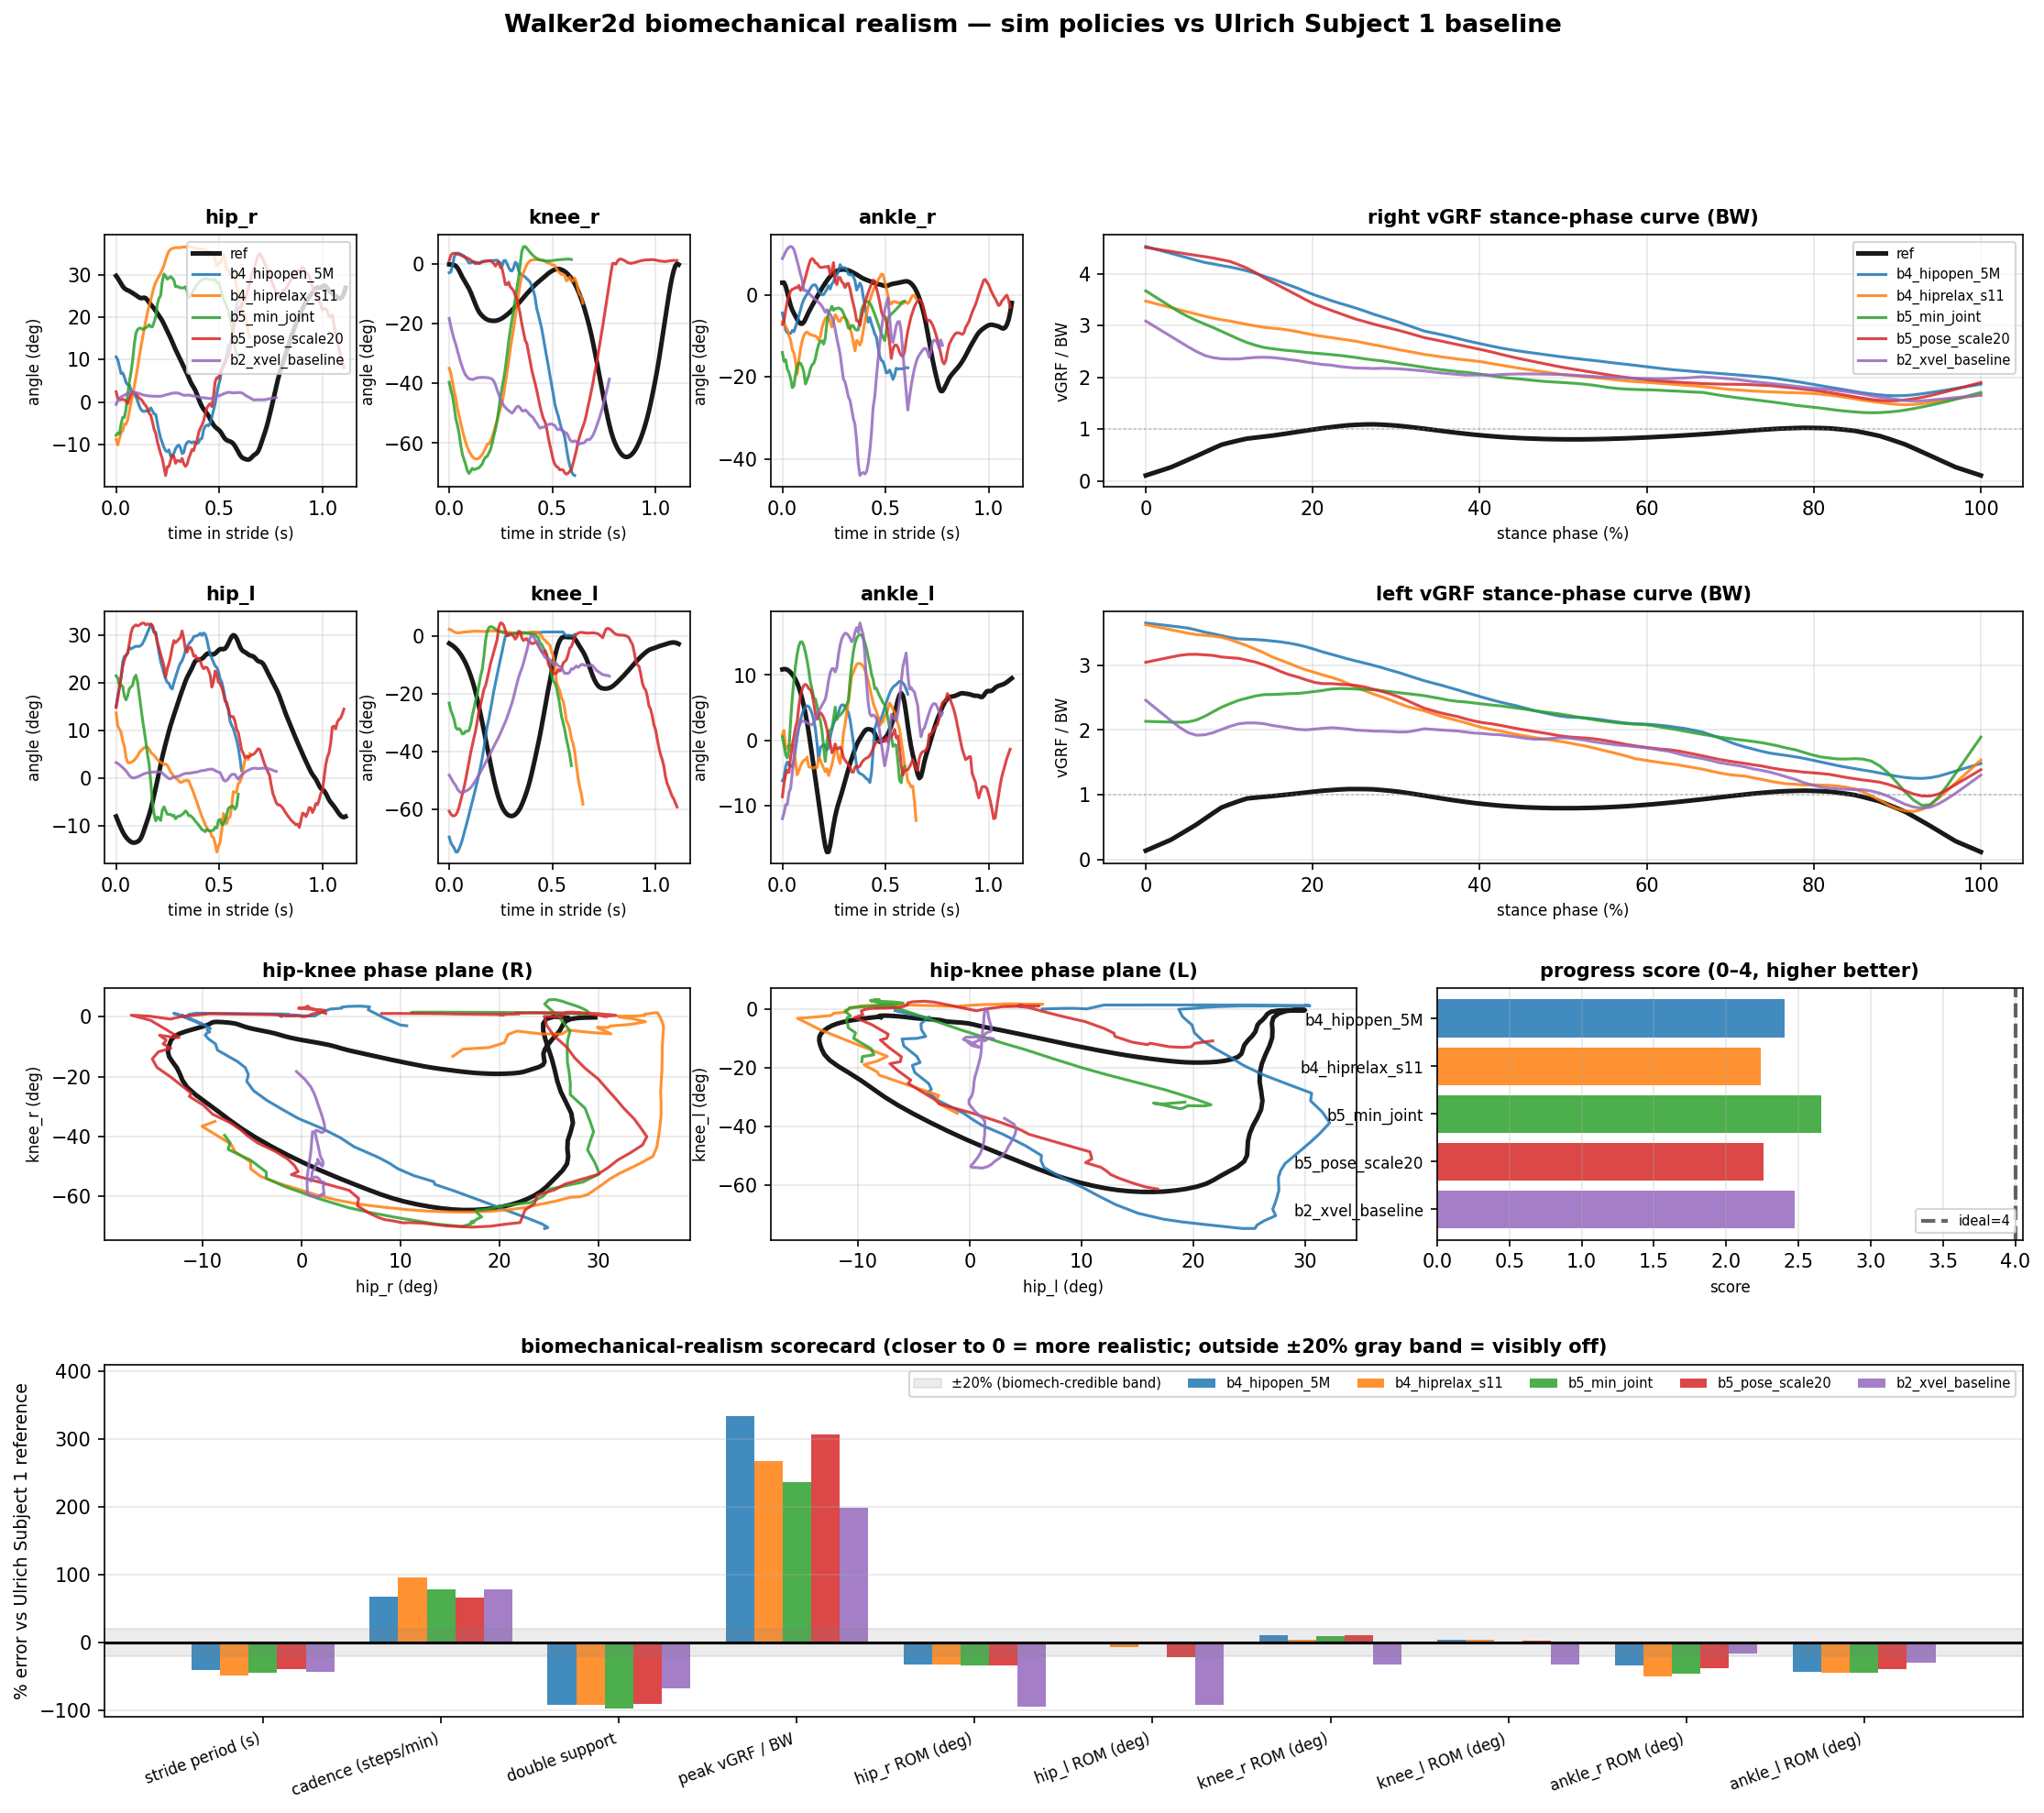
\includegraphics[width=0.97\textwidth]{biomech_dashboard.png}
\caption{Held-out biomechanical-realism scorecard. \textbf{Top two rows:} bilateral kinematics for hip, knee, and ankle, plus left and right vertical ground reaction force across stance phase. Reference (Subject 1, Ulrich baseline at 1.25\,m/s) is the bold black trace. \textbf{Third row:} hip--knee phase planes (R, L) and progress-score bars in $[0, 4]$. \textbf{Bottom row:} \% deviation from reference per metric, with $\pm 20$\,\% credible band shaded. Joint kinematics qualitatively track the reference; peak vGRF is 3--4 body weights vs.\ a measured 1.10 BW, and double-support fraction collapses to roughly 1\,\% vs.\ a measured 23\,\%.}
\label{fig:dashboard}
\end{figure}

The progress score (Fig.~\ref{fig:dashboard}, right of third row) aggregates the per-metric deviations against a $\pm 20$\,\% credible band; the lead policy lands at 2.66 of a possible 4.0, with the alternative candidates between 2.24 and 2.40. The pre-MJCF-fix baseline (\texttt{b2\_xvel}, trained against the stock thigh range) scores 2.47---only marginally lower than the post-fix candidates. Three rounds of reward and termination tuning, plus the kinematic-ceiling fix, did not move the policy off the same biomechanical-quality floor.

The reading is straightforward: the multi-term DeepMimic reward optimizes pose, velocity, end-effector position, root height, and contact alternation. It does not optimize peak vGRF, double-support fraction, or joint ROM amplitude. The policy is exactly as biomechanically realistic as the reward asks it to be. \textbf{This is Goodhart's Law at the top level of the reward: the policy walks the way the reward was written, not the way humans walk.} Closing the remaining gap inside this paradigm would require explicitly engineering vGRF, DSF, and ROM targets into the reward---which is hand-engineering walking, the opposite of imitation. \textbf{H2 is confirmed.}

\subsection{AMP at small environment counts collapses (H3 confirmed)}
\label{sec:results-amp}

We trained AMP at the same 8-CPU-environment scale for 20\,M steps. The style reward $r_s$ converges to $0.028$--$0.034$ rather than the $r_s \in [0.5, 1.0]$ range that would indicate meaningful style matching. The rendered final policy produces worse walking than the engineered baseline: the near-zero style reward provides insufficient gradient signal to shape the gait, and the task reward alone (forward velocity) optimizes speed without kinematic structure.

The collapse mechanism is as follows. With 8 environments and \texttt{n\_steps}=2048, each rollout provides $8 \times 2047 = 16{,}376$ policy transitions. The expert buffer contains 349 transitions drawn from the 350-frame reference cycle. In the 24-dimensional discriminator input space, early-training policy transitions cluster near the initialization distribution while expert transitions form a compact 1-D manifold (the gait cycle). A discriminator with even 64 hidden units can achieve near-perfect separation before the policy has produced any meaningful walking, driving $r_s \to 0$ and eliminating the style gradient. Expert noise ($\sigma = 0.05$\,rad) and the zero-centered gradient penalty partially slow this process but cannot prevent it at this scale.

The original AMP paper~\cite{escontrela2022amp} ran 4096 parallel environments on a GPU cluster. At that scale, policy transitions are diverse enough to prevent the discriminator from memorizing the compact expert manifold; the discriminator must generalize rather than memorize. With 8 environments, this diversity is structurally unachievable regardless of discriminator capacity or regularization. AIRL behaves similarly at small scale, with the shaping potential providing slightly more stable gradients early in training but the final policy still under-performing the engineered baseline. \textbf{H3 is confirmed.}

\section{Conclusion and Future Work}
\label{sec:conclusion}

We trained a phase-conditioned PPO policy on real human IK data with a DeepMimic-style multi-term imitation reward, reference-state initialization, and a PD-rollout behavioral cloning warm-start, on a 2D torque-actuated MuJoCo Walker2d. Training is stable, the policy survives multi-thousand-step rollouts, and the rendered video is visually plausible. A held-out biomechanical-realism scorecard built from the subject's measured force plate and IK then reveals that the policy is not biomechanically realistic on the kinetic axes the reward leaves unspecified: peak vGRF is 3--4$\times$ the reference, double-support fraction collapses to roughly 1\,\% versus 23\,\%, and joint ROM amplitudes under-shoot by 30--50\,\% at the hip and ankle. The policy walks the way the reward was written. Three rounds of reward and termination tuning did not change this; a parallel AMP implementation at the same scale collapses for an orthogonal reason (discriminator memorization on a compact expert manifold).

What we learned: \textbf{visual plausibility is a misleading evaluation criterion for gait imitation}. Held-out biomechanical metrics are essential, and they expose a structural limitation of engineered-reward imitation on a torque-actuated 2D walker: every dimension the reward does not explicitly target is one the optimizer is free to escape on. Closing the remaining gap inside the engineered-reward paradigm amounts to engineering walking by hand, which defeats the imitation premise.

\paragraph{Future work, framed as the two natural responses to this finding:}
\begin{enumerate}\setlength\itemsep{1pt}
    \item \textbf{Adversarial imitation at GPU scale.} Port \texttt{Walker2dPhaseAware} to MuJoCo MJX (JAX GPU backend) targeting 2{,}000--4{,}000 parallel environments on a single GPU, reproducing the conditions under which~\cite{escontrela2022amp} ran AMP successfully and~\cite{rudin2022walk} demonstrated minutes-rather-than-hours legged-locomotion training. At that scale, policy diversity itself prevents the discriminator from memorizing the compact expert manifold, and the style gradient becomes informative. The negative result on engineered rewards reported here \emph{strengthens} the case for moving the AMP/AIRL track to GPU scale rather than continuing to tune the engineered reward.
    \item \textbf{Return to muscle-actuated dynamics.} The original proposal scoped a 3D, 80-muscle, 20-DoF MyoLeg agent~\cite{caggiano2022myosuite} precisely because muscle dynamics couple kinematics and kinetics through physiology rather than reward weights. Hill-type muscles cannot generate arbitrary peak vGRF without exceeding force-length-velocity limits, and they enforce smooth force production through activation dynamics. In that substrate, biomechanical realism may be the path of least resistance rather than something the reward must enforce by hand. Our 2D torque-actuated negative result is empirical motivation for that scope, not a reason to abandon it.
\end{enumerate}

Beyond these two paths, multi-cycle and multi-subject reference data would address the smoothness and over-fitting limits of the single-cycle reference, and a multi-step preview observation $[q^{\text{ref}}_\phi, q^{\text{ref}}_{\phi+1}, \ldots, q^{\text{ref}}_{\phi+K-1}]$ may help the policy anticipate phase transitions when the reward signal is weak.

\paragraph{Code.} \url{https://github.com/Brock-Perreca/6955_Project}

\bibliographystyle{plain}
\bibliography{references}

\end{document}
